%!TEX root = ..\..\dissertation.tex
\section{On Platforms}
Platforms are a way to manage variety by allowing certain areas or features of a product or system to be changed, while standardising and effectively ``locking'' other features. 
They are essentially a collection of decisions on certain aspects of a system, which designers and developers must adhere to when creating a new system.
These decisions can be made for various purposes, \eg{} to ensure compatibility between system generations, speed up the system design process, ensure system robustness, ease integration of new technology, or guarantee manufacturability, to mention a few.
Standardisation of physical and non-physical assets, as well as the sharing of these assets or characteristics, \ie{} \gls{glos:cmmnlty}, is the core of platforms.
In this way, new system variants and generations can relatively quickly be created by designers and developers utilising platforms.
As such, platforms are the result of answering two essential questions with regards to a system~\parencite{SorensenMCPC2017}:
\begin{itemize}
	\item What may change and what may not?
	\item Where is variety acceptable and where is it not?
\end{itemize}
One area where platforms have seen significant success is in product design and development, where they have been successfully adopted to manage an increasing number of product variants~\parencite{AIE:276705}.
While various definitions pertaining to platforms exist, this thesis subscribes to the definition proposed by~\textcite{MeyerLehnerd}.
\begin{definition}{\gls{glos:platform}}
a collection of elements and interfaces forming a common structure, from which a stream of derivative products can be efficiently developed~\parencite{MeyerLehnerd}
\end{definition}
This makes the platform itself distinct from another commonly used term in product design and development; product family.
Where a platform is a collection of entities from which products are built, a product family is a collection of products sharing certain common characteristics, which may have been built on a platform.
The definition above was originally aimed towards products (\ie{} product platforms), but it is also considered pertinent when discussing manufacturing systems, as these are considered the product of a targeted design and development process, and a technical product can generally be considered a system.
Research in the development, implementation, and utilisation of manufacturing system platforms is sparse and examples are few~\parencite{BossenPbCd,SorensenAPMS2018}, but several well-known aspects of product platforms can be applied to manufacturing system platforms as well.
Among these are the core concepts of architecture, modules, interactions, and interfaces.

\subsection{Architecture}
The concept of system \gls{glos:arch} is similar to that of platforms, and the two terms are often used interchangeably despite significant differences between the two.
In system design and development, regardless of whether these systems are products or manufacturing systems, an architecture is essentially a description of a system or system of systems.
It captures both the functional and physical elements of a system, how they relate to each other, and how the system interacts with its environment.
Where a platform contains the standardised elements or features upon which systems can be or are built, the architecture contains all elements and relations of a system, including those that are not standardised~\parencite{HarlouU}.
As such, a platform can be considered a subset of an architecture.
However, while all systems exhibit an architecture (explicit and intentionally developed or otherwise), not all systems exhibit platforms.
Architectures are commonly used within systems engineering and software development~\parencite{9781118999400,ISO42010}.
This thesis aligns itself with a slightly modified definition of architecture by \textcite{UlrichEppinger}, relying on the notion of modules discussed in the following section.
\begin{definition}{\gls{glos:arch}}
the architecture of a system is the scheme by which the functional elements of the system are arranged into modules and by which the modules interact
\end{definition}

\subsection{Modules}
Platforms and modules are closely related, but remain distinct concepts~\parencite{DitlevModDrivers}.
A module is an entity designed to implement one or more well-defined functions, with well-defined interfaces connecting one module to another.
Examples of various common types of modularity are shown on \cref{fig:typesModularity}.
\begin{figure}[tb]
	\centering
	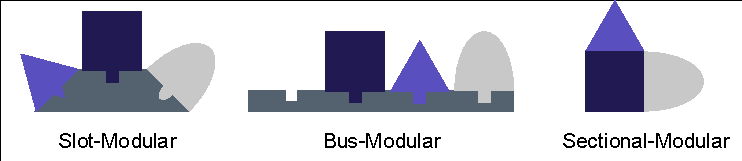
\includegraphics[width=.8\textwidth, trim=3 3 3 3, clip]{mainmatter/introduction/figures/modularity.pdf}
	\caption[Three common types of modularity.]
	{Three common types of modularity.
	Redrawn from \textcite{UlrichEppinger}.}\label{fig:typesModularity}
\end{figure}
This aligns with the core purposes of a platform, since modules are essentially standardised assets, functions, and interfaces.
Platforms are characterised by a particular type of modularity, as the constituents of a platform are elements with low variety and high reusability~\parencite{BaldwinWoodard2009}, making platforms modular by nature.
Systems based on platforms will typically be constructed from these platform modules of low variety and high reusability, combined with a number of modules with high variety and low reusability in order to create the desired variety of the system.
There can be a number of reasons for why a module exists or why a particular set of functions are encapsulated in a single module.
These are generally dubbed module drivers, and represent different criteria behind modularisation~\parencite{Erixon19961}.
Although the module drivers were originally defined for product design and development, \textcite{DitlevModDrivers} identified several drivers applicable within production and manufacturing system design, as outlined in \cref{tab:modularDrivers}.
\begin{table}
	\centering
	\caption[Relevant drivers for modular production.]
	{Relevant drivers for modular production.
	Adapted from \parencite{DitlevModDrivers}.}\label{tab:modularDrivers}
	\small
	\begin{tabular}{p{.16\textwidth}p{.27\textwidth}p{.4\textwidth}}
		\toprule
		Category & Driver & Description\\
		\midrule
		\multirow{3}{.2\textwidth}{System Development} & Geometric Integration and Precision & Careful alignment of parts and manufacturing assets.\\
		& Function Sharing & Two or more manufacturing assets sharing a common function.\\
		& Portability of Interfaces & Ease of connecting two manufacturing assets via an interface.\\
		\midrule
		\multirow{3}{.2\textwidth}{Localization of Changes} & Module Carryover & Functions not expected to change in the future.\\
		& Technology Evolution & Changes expected due to implementation of new manufacturing technology.\\
		& Planned Product Changes & Planned changes due to product/production planning.\\
		\midrule
		\multirow{2}{.2\textwidth}{Variety and Standardisation} & Common Unit & Function required by several different manufacturing assets.\\
		& Different Specification & Function required for localised differentiation.\\
		\midrule
		Production of Manufacturing equipment & Vendor Capabilities & Outsourced functions.\\
		\midrule
		Service and Recycling & Service and Maintenance & Frequently used functions subject to wear.\\
		\bottomrule
	\end{tabular}
\end{table}


\subsection{Interfaces \& Interactions}
To describe how systems and their elements interact and are influenced by each other and the environment, the terms interaction and interface will be used.
An \gls{glos:interaction} is some effect that occurs between at least two objects, while an \gls{glos:interface} is how said effect is transferred from one object to another.
The distinction between these two is often overlooked, as the focus is typically on interfaces, which tend to cover both terms in one.
It is, however, an important distinction to make when it comes to platform development in order to identify similar interactions carried out over different interfaces.
\begin{definition}{\gls{glos:interaction}}
a mutual or reciprocal action occurring as a result of two or more objects influencing each other
\end{definition}
\begin{definition}{\gls{glos:interface}}
a point of contact between two or more objects, at and/or through which an interaction occurs
\end{definition}

Interactions are further classified into four generic types; spatial, energy, information, and material~\parencite{Pimmler94integrationanalysis}.
A spatial interaction calls for adjacency, orientation, or alignment, \eg{} two parts oriented for assembly, or a gripper being adjacent to the end of an articulated robot.
An energy interaction describes a need for energy transfer, \eg{} the transfer of heat from a processor to a heatsink, or power from a power supply to components in a control system.
An information interaction identifies a need for information, data, or signal exchange, \eg{} exchange of information between a sensor and a control system or processor.
A material interaction calls for material exchange, \eg{} airflow over a heatsink or water from a pump to a pipe system.
Individual interfaces can facilitate multiple interactions depending on the level of detail being considered.
In the case of the interaction between the heatsink and processor described above, there is also a need for a physical contact and alignment (\ie{} a spatial interaction) between the two components.
Such interactions between heatsink and processor can be realised in various manners.
Screws and pins can be used to align the two components, while a thermal interface material (such as cooling paste) can be used to facilitate the transfer of heat and absorb tolerances from spatial alignment.
Fans attached to the heatsink can then provide an increased airflow for a material interaction, and the processor can be connected to a sensor and power supply through wires or pins on a motherboard for energy, information, and spatial interactions.

\subsection{Manufacturing System Platforms and Changeable Manufacturing}\label{ssec:pPlatforms}
Development and utilisation of platforms in manufacturing is an enabler for changeable manufacturing; a way to improve variety management in manufacturing systems.
Changeable manufacturing is a manufacturing paradigm based on the concept of \gls{glos:changeability}, \ie{} the characteristics giving manufacturing systems the capability to accommodate to change in an economical manner by making adjustments at all levels of a factory~\parencite{HodaC}.
It is an umbrella term encapsulating a number of so-called \gls{glos:changeability} classes, each relating to specific levels within a factory, as shown on~\cref{fig:chngbltyClasses}.
Each level, when broken down, consists of one or more instances on the lower level, \eg{} a network consisting of multiple factories, a factory consisting of multiple segments, and a segment consisting of multiple manufacturing systems.
\begin{figure}[tb]
	\centering
	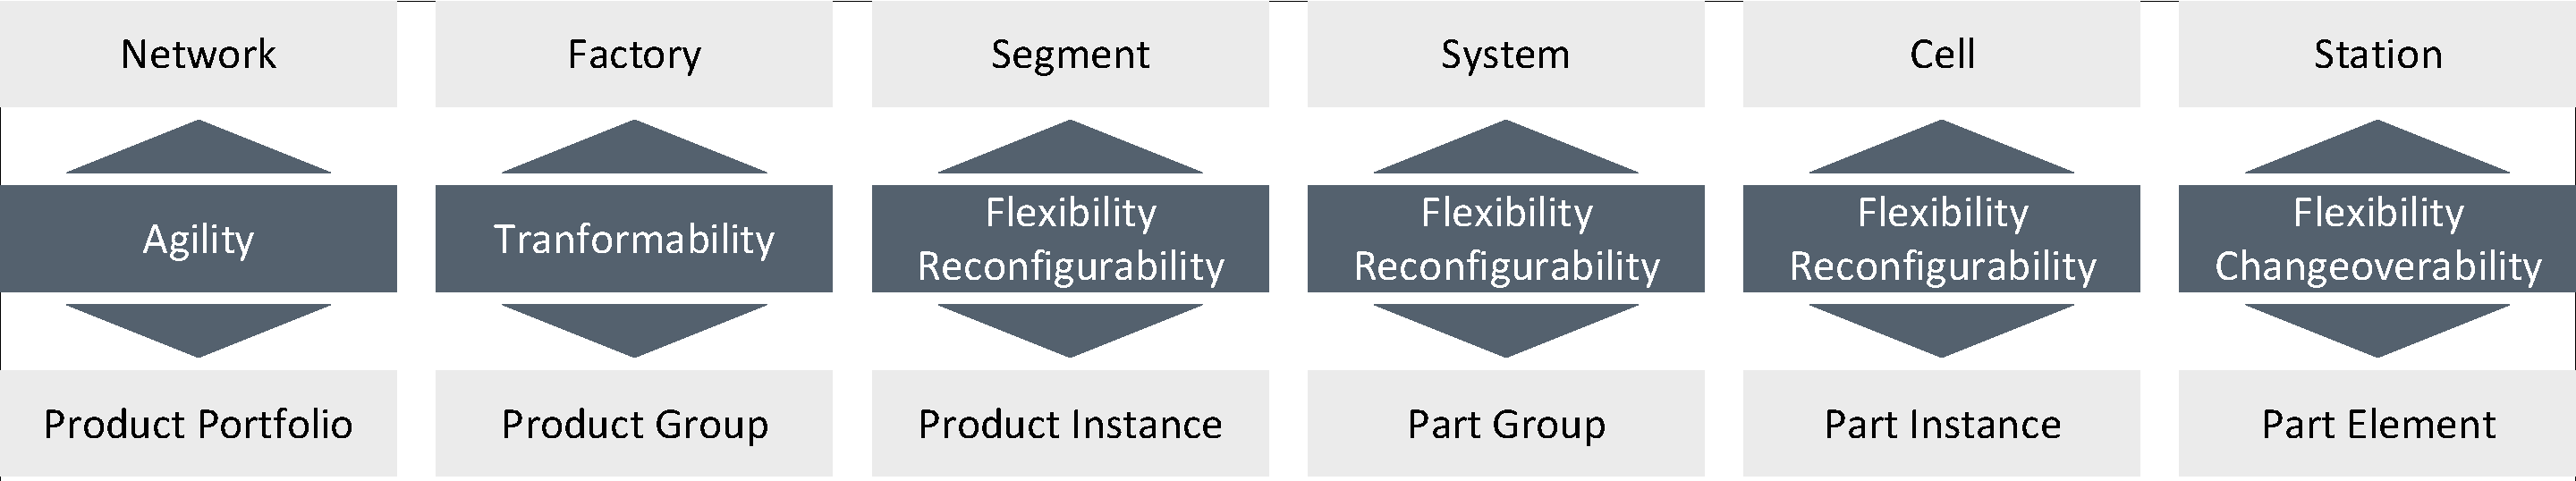
\includegraphics[width=\textwidth, trim=3 3 3 3, clip]{mainmatter/introduction/figures/factoryLevels.pdf}
	\caption[The six levels of a factory, their corresponding changeability class and equivalent product level.]
	{The six levels of a factory (top), with their corresponding changeability class (mid), and the equivalent product level (bottom).
	Adopted from \textcite{HodaC}.}\label{fig:chngbltyClasses}
\end{figure}
The five changeability classes are briefly outlined below~\parencite{HodaC}:
\begin{itemize}
	\item \textbf{Agility:} strategic ability of a company to respond to volatile market conditions, \eg{} by pursuing new markets, services, products, or manufacturing systems.
	\item \textbf{Transformability:} tactical ability of a factory to switch between a variety of product groups or families.
	\item \textbf{\Gls{glos:reconf}:} ability of a production area to, through a physical change, switch between similar product groups or families with relative ease and speed.
	\item \textbf{Flexibility:} operative ability of a production system to, without a physical change, switch between variants within a predefined product family quickly and effortlessly.
	\item \textbf{Changeoverability:} operative ability of a workstation to perform specific operations without effort and delay.
\end{itemize}
Traditional dedicated manufacturing systems (DMS), lacking the characteristics facilitating change, are unable to keep up with the rapid introduction of new technologies, products, and variants.
Changeable manufacturing systems (\gls{glos:CMS})---\ie{} manufacturing systems possessing characteristics giving them the capability to accommodate change---and in particular reconfigurable manufacturing systems (\gls{glos:RMS}) are becoming increasingly relevant to manufacturers.
One of the key characteristics of \gls{glos:RMS} is modularity~\parencite{Koren,HodaC}.
The modular nature of both platforms and RMS implies a connection between the two.
In fact, the utilisation of platforms to design an RMS can be considered part of the basic and advanced design phases of RMS design.
Following \posscite{Andersen2017179} generic method for RMS design, platforms can play into the basic design phase when realisation of \gls{glos:reconf} and functionality is determined, interfaces identified and specified, and system elements are decided upon.
A simplified illustration of the design approach is shown on \cref{fig:pltfRMS}, with highlights added to illustrate when platforms can provide a benefit.
For the advanced design phase, the platform plays into the detailing of system modules, system interfaces, and detailed manufacturing equipment design.
These functional elements, enablers, interactions, interfaces, and modules are all things a platform should include.
\begin{figure}[tb]
	\centering
	\makebox[\textwidth][c]{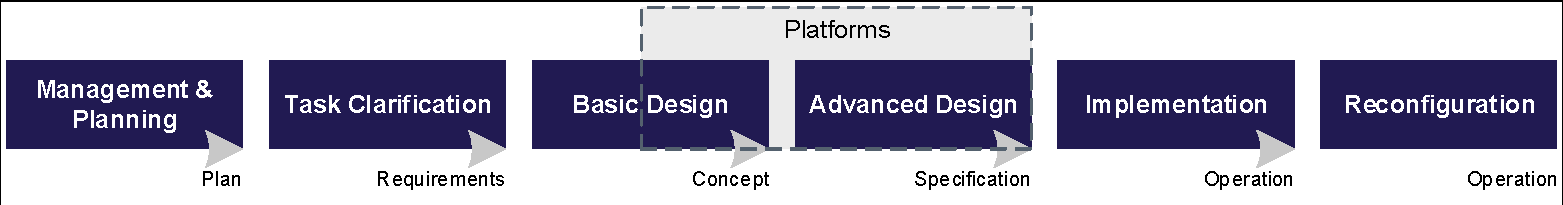
\includegraphics[width=1.1\textwidth, trim=2 2 2 2, clip]{mainmatter/introduction/figures/genericRMS.pdf}}
	\caption[Generic reconfigurable manufacturing system design approach.]
	{Simplified generic reconfigurable manufacturing system design approach by \textcite{Andersen2017179}.
	A dashed box has been highlighted to during which stages utilisation of platforms provide the largest benefit~\parencite{SorensenCMS2019}.}\label{fig:pltfRMS}
\end{figure}

With the development, implementation, and utilisation of manufacturing system platforms remaining a relatively immature field of research, attempts at drawing inspiration, concepts, and methods from other areas where maturity is higher and platforms are more common have previously been made, especially borrowing from software architecture and development~\parencite{SorensenMCPC2017,BENKAMOUN201488,JepsenPhD,BossenCMod}.
Having both a product and manufacturing system platform available could greatly limit the effects of introducing a new product variant or generation, preventing these changes from propagating throughout a manufacturing company.
Utilising both types of platforms in conjunction facilitates co-development of new solutions across departments in a manufacturing company.